\documentclass[10pt,a4paper]{article}
\usepackage[utf8]{inputenc}
\usepackage{amsmath}
\usepackage{amsfonts}
\usepackage{amssymb}
\usepackage{graphicx}
\usepackage{placeins}

\begin{document}

\section*{Thermodynamics Scratch Sheet}


	\begin{figure}[h]
		\centering
		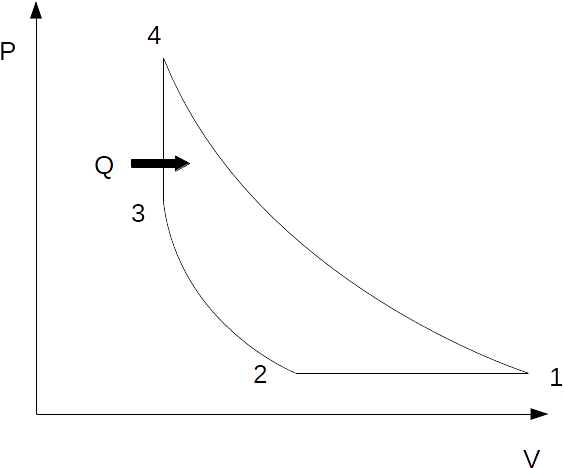
\includegraphics[width=.5\textwidth]{ThermoDiagram.png}
		\caption{PV Diagram of Modern Atkinson Cycle}
		\label{fig:diagram1}
	\end{figure}
	The engine has 6 cylinders and 3000 c.c. total swept volume. The fuel used will be standard octane gasoline. Intake is taken from the ambient atmosphere.\\
	A modern atkinson cycle is chosen in-lieu of the traditional Otto cycle for it's increased ideal efficiency and better mixing properties.\\
	These parameters completely define our thermal cycle. Since the proportion of gasoline is small, and gasoline composed of nonpolar substances, an air standard model is used. The air is not assumed cold - the cold assumption results in far too significant of errors. NASA empirical air curves are used instead.
	\subsection*{Initial Constraints}
	Our compression ratio is taken to be 10, a high compression ratio that prevents knocking. \\
	A lean air to fuel mixture ratio of 29.4 is chosen to ensure complete combustion and limit the pressures.
	\begin{align}
		C_R &= \frac{V_1}{V_2} \\
		M_R &= \frac{m_A}{m_G} = 29.4
	\end{align}
	The volumes are constrained by the total c.c. of the engine. Likewise, it is noted process 3-4 is isochoric.
	\begin{align}
		\frac{3000\ \text{c.c.}}{6} &= V_4-V_2 
	\end{align}
	Finally, point 1 and point 2 are at ambient pressure $p_{amb}$, temperature $T_{amb}$, and density $\rho_{amb}$. Also calculations will use a reference STP density $\rho_o$ and $T_o$. Likewise the gas constant for air is used.
	\begin{align}
		R_A &= 287.1 \\
		p_{amb} &= 101325\ \text{Pa} \\
		T_{amb} &= 288\ \text{K} \\
		\rho_{amb} &= 1.225\ \text{kg}\ \text{m}^{-3}\\
		T_o &= 273.15\ \text{K} \\
		\rho_0 &= 1.2754\ \text{kg}\ \text{m}^{-3}
	\end{align}
	The lower value of the heat of combustion from the U.S. EIA.
	\begin{align}
		H_G &= 46.7\ \text{MJ}\ \text{kg}^{-1}
	\end{align}
	\subsection*{State 1}
	This is the start of the compression stroke right after the intake stroke. The air is at ambient conditions, noted in the previous section. Additionally the specific volume is calculated and the internal energy taken from an air table.
	\begin{align}
		u_1 &= 205.71\ \text{kJ}\ \text{kg}^{-1}\\
		v_1 &= 0.8163\ \text{m}^3\ \text{kg}^{-1}
	\end{align}
	
	\subsection*{State 2}
	The process from state 1 to state 2 is an isentropic process.
	\begin{align}
		C_R &= \frac{v_1}{v_2}\\
		v_2 &= \frac{v_1}{C_R}\\
		v_2 &= 0.08163\ \text{m}^3\ \text{kg}^{-1}\\
		\rho_2 &= 12.25\ \text{kg}\ \text{m}^{-3}
	\end{align}
	Since it's an isentropic process, the final state can be found from the air table.
	\begin{align}
		T_2 &= 703\ \text{K}\\
		u_2 &= 514.95\ \text{kJ}\ \text{kg}^{-1}
	\end{align}
	\subsection*{State 3}
	The process from state 2 to state 3 is an isochoric process with an input Q. The specific heat is given by the mass ratio.
	\begin{align}
		m_t &= m_G + m_A = m_G + M_R m_G \\
		Q &= m_G H_G \\
		q &= \frac{Q}{m_t} = \frac{H_G}{1 + M_R}\\
		q &= 1.5362\ \text{MJ}\ \text{kg}^{-1}
	\end{align}
	W = 0, so our final internal energy is given by adding the heat and initial internal energy.
	\begin{align}
		u_3 &= q + u_2\\
		u_3 &= 2051.1\ \text{kJ}\ \text{kg}^{-1}
	\end{align}
	The density is the same as before, since it's an isochoric process. Additional properties are now derived from the air table.
	\begin{align}
		p_3 &= 8.187\ \text{MPa}\\
		T_3 &= 2385\ \text{K}\\
		\rho_3 &= 12.25\ \text{kg}\ \text{m}^{-3}\\
		p_{3r} &= 4443.2
	\end{align}
	\subsection*{State 4}
	This is the expansion stroke - modeled as an isentropic process. The pressure it expands to is chosen so enough power is produced.
	\begin{align}
		p_4 &= 2.25 p_o = 227.98\ \text{kPa}\\
		p_{4r} &= 123.73
	\end{align}
	Since it's an isentropic process, the relative pressure can be used to find the final properties.
	\begin{align}
		T_4 &= 1022\ \text{K}\\
		u_4 &= 778\ \text{kJ}\ \text{kg}^{-1}\\
		\rho_4 &= 0.777\ \text{kg}\ \text{m}^{-3}
	\end{align}
	\subsection*{Total Cycle Analysis}
	The isentropic processes have no heat transfer - $W = \Delta U$.\\
	The isochoric processes have no work.\\
	The isobaric process has a simple work relation - $W = P \Delta V$.\\
	Our specific work is given below:
	\begin{align}
		w_{cyc} &= (u_3-u_4) - (u_2-u_1) - p_{amb}(v_4 - v_1) \\
		w_{cyc} &= 916.17\ \text{kJ}\ \text{kg}^{-1}
	\end{align}
	The total air mass per cylinder can now be found:
	\begin{align}
		\frac{3000\ \text{c.c.}}{6} &= m_t(v_4-v_2)\\
		m_t &= 414.81E-6\ \text{kg}
	\end{align}
	Finally, one total cycle is completed per piston for every 2 rotations. The power is given by the mass, specific work, and rotational frequency. The power is evaluated at 8000 R.P.M.
	\begin{align}
		P &= 6 m_t w_{cyc} \frac{f}{2}\\
		P &= 152.01\ \text{kW}\\
		P &= 203.85\ \text{hp}\\
		\eta &= \frac{w_{cyc}}{q}\\
		\eta &= 59.6 \%
	\end{align}
\end{document}